%AUTORIZACIÓN BASADA EN ROLES
%La autorización o el control de acceso basado en roles permite establecer y hacer cumplir los permisos que tienen un conjunto de usuarios pertenecientes a un rol, de acceder a un recurso del sistema. Cuando se habla de acceso a un recurso, se refiere a acciones de lectura, escritura, ejecución, modificación. A diferencia de establecer listas de control de acceso para cada recurso del sistema, se define una lista de privilegios o permisos para los diferentes roles. Los roles son definidos, a través de la agrupación de características de los usuarios del sistema.

\chapter{Métodos para la autenticación central}\label{chapter:state-of-the-art}
En este capítulo se brindan las definiciones de herramientas utilizadas para la autenticación. También se realiza un estudio sobre el estado del arte de las mismas. Además, se brindan razones para incluir su utilización como parte de la solución propuesta.

\section*{Autenticación y Autorización}
La autenticación y la autorización son los primeros parámetros de seguridad que las aplicaciones web consideran para protegerse de accesos no autorizados [\cite{deitel2014como}].  Aunque los dos términos aparecen a menudo en el mismo contexto, los dos son conceptualmente muy diferentes. Autenticar es confirmar una identidad, mientras autorizar significa dar acceso a un sistema. En pocas palabras, la autenticación es el proceso de verificar una identidad y la autorización es el proceso de verificar que tiene acceso [\cite{ye2022diseno}].

\subsection*{Autenticación}
La autenticación consiste en validar credenciales, como nombre de usuario/correo electrónico y contraseña, para verificar la identidad del visitante. El sistema determina si el usuario está usando las credenciales correctas. Tanto en redes públicas como privadas, el sistema autentica al usuario a través del inicio de sesión y generalmente se realiza mediante un nombre de usuario y
una contraseña. Sin embargo, la autenticación puede realizarse  también a través de otros factores como el código de verificación de teléfonos móviles o datos biométricos.

En algunos sistemas de aplicaciones, para lograr una mayor seguridad, requieren el uso conjunto de múltiples factores de autenticación, a menudo llamado \textit{Multifactor Authentication}.

hablar de los tipos de autenticacion

explicar autenticacion basada en tokens 

explicar JWT


%hay más info en  [\cite{ye2022diseno}].
%Se han definido métodos generales de autenticación web que han sido desarrollados a lo largo del tiempo: Autenticación de factor único [\cite{mendoza2020importancia}], Autenticación de doble factor [\cite{lopez2019herramienta}], Autenticación gráfica [\cite{rodriguez2018seguridad}], Autenticación por token [\cite{rodriguez2018seguridad}], Autenticación biométrica [\cite{mantovani2019autenticacion}].

%\subsection{Tipos de Inicio de Sesión Único}
%The various types of SSO shown in Fig: 1, fall under different categories, based on where they are deployed (Intranet, Extranet, Internet); how they are deployed (architecture – Simple, Complex); the credentials they use (token, certificate..) and the protocols they use (Kerberos, SAML, OpenID..).Following picture shows the types of SSO and their classification: 
%
%\begin{figure}[H]
%	\centering
%	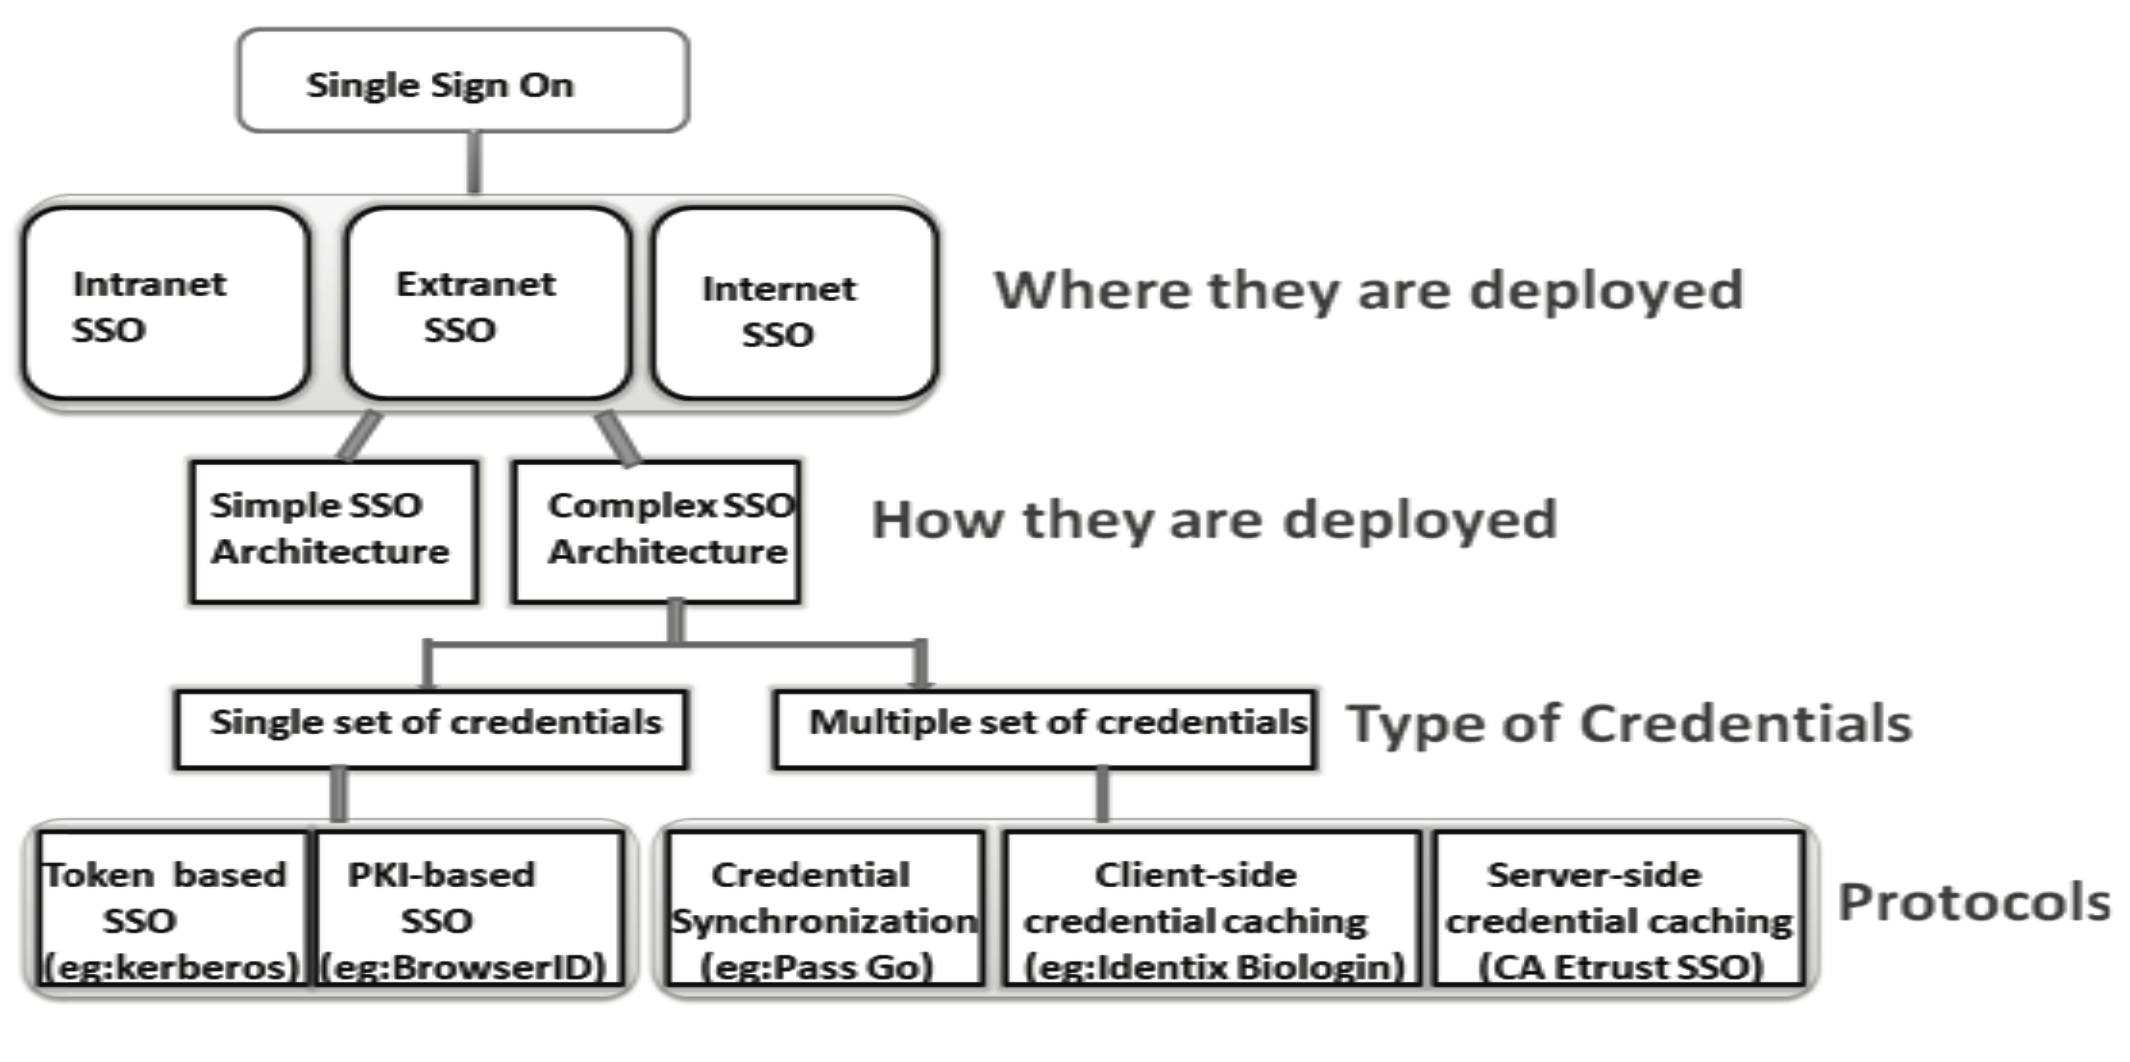
\includegraphics[width=0.7\linewidth]{Graphics/sso_types}
%	\caption{}
%	\label{fig:Tipos de SSO}
%\end{figure}
%
%Dadas las condiciones de la Universidad, se despliegará en Extranet ya que \textcolor{red}{Multi-domain SSO allows connecting to multiple systems within the same enterprise and all the business partners’ applications. The user can login into one enterprise and access resources of the other, the users need not login again using different credentials.}
%
%Se despliegará con una arquitectura de tipo SSO compleja ya que \textcolor{red}{Complex SSO uses multiple authentication authorities with single or multiple sets of credentials for each user.}
%
%En este caso se utilizarán un único conjunto de credenciales basado en tokens porque \textcolor{red}{In this SSO system, a user submits the credentials to the token-based authentication authority, in which the credentials have been checked with its credential database. If the user credentials match, then the user is returned with a token. When the user wants to access an application server which is governed by second authentication authority, the same token is delivered to get a ticket to access the application server. Success of this process relies on the trust the authentication authorities have among themselves.}

%[\cite{radha2012survey}]

\subsubsection*{Autenticación basada en tokens}

Los tokens de acceso se utilizan en la autenticación basada en tokens para permitir que una aplicación acceda a una API. Cuando un usuario se autentica y es autorizado correctamente, la aplicación recibe un token de acceso que luego utiliza como credencial cuando llama a la API. El token pasado informa a la API que el portador del token ha sido autorizado para acceder y realizar un grupo de acciones. [\cite{auth0AccessTokens}]

%\textcolor{red}{tipos de tokens: https://auth0.com/docs/secure/tokens/access-tokens}

Un token consiste en datos relacionados con la identidad de un usuario particular. Los usuarios pueden obtener dichos tokens a través de una combinación de nombre de usuario/contraseña, lo que les permite acceder a los recursos solicitados por un periodo específico de tiempo. Durante este periodo no se requieren métodos adicionales de autenticación. Una característica importante de los tokens es que permiten ser heredados a otros usuarios, por ello, la autenticación basada en tokens es adecuada cuando un token puede proveer acceso a múltiples servicios. [\cite{banerjee2018token}] %esta bib tiene más info: banerjee2018token, tecnicas

Existen diversos protocolos de autenticación basados en tokens, los más populares son: SMAL 2.0 [\cite{cantor2005assertions}]; OpenID [\cite{recordon2006openid}] [\cite{mainka2017sok}] y OAuth [\cite{hardt2012oauth}] [\cite{richer2017oauth}]. 

Tokens are system generated arbitrary construct that asserts the identity of what it claims to be [\cite{zheng2014token}]Token-based authentication embodies the exchange of client authentication credentials for a server generated authentication token; and for subsequent client requests to access SaaS resources, the tokens are sent as part of the request in the HTTP header to the server. This reuse of the same user access token for accessing protected resources governed by certain policies can be a challenge, especially when a resource access policy is updated and the user access token is still valid. In fact, this can introduce a Time- Based vulnerability (timing attack) on the protected resources; and with multiple users accessing the resource, the vulnerability index can increase exponentially. Hence, an authentication and authorization model that limits such vulnerabilities and enhances secure resource access have been proposed and evaluated. [\cite{ethelbert2017json}]

\subsection*{Autorización}
La autorización ocurre después de que el sistema completa la autenticación. Es el proceso de determinar si un usuario autenticado puede acceder a un recurso en particular. Verifica que está autorizado para otorgarle acceso a recursos tales como información, bases de datos, archivos, etc.

\begin{table}[H]

\centering
\begin{tabular}{ |p{4cm}| p{4cm} | }
	\hline
	 \textbf{Autenticación}&\textbf{Autorización}\\
	\hline
	Confirma la identidad para otorgar acceso al sistema & Determina si tiene acceso a un recurso\\
	\hline
	Este es el proceso de validación de credenciales de usuario para obtener acceso de usuario&Este es el proceso de verificar que el acceso está permitido\\
	\hline
	Generalmente requiere un nombre de usuario y una contraseña& Los factores de autenticación son necesarios para que la autorización pueda variar según el nivel de seguridad\\
	\hline
	La autenticación es el primer paso & La autorización se realiza después de una autenticación exitosa\\
	\hline
\end{tabular}
\caption{\label{tab:table-name}Comparación entre autenticación y autorización.}
\end{table}

\section*{Inicio de Sesión Único}
El Inicio de Sesión Único ( en inglés \textit{Single Sign-On} o también conocido por sus siglas SSO) ha sido ampliamente adoptado para la autenticación en línea debido a su utilidad y la seguridad que ofrece. Este es un método de autenticación que permite a los usuarios iniciar sesión con un único conjunto de credenciales en varios sistemas independientes. El inicio de sesión único facilita que un usuario no tenga que iniciar sesión en cada aplicación que use. Con este servicio los usuarios pueden acceder a todas las aplicaciones necesarias sin tener que autenticarse con otras credenciales.[\cite{microsoft-doc}]

En el mundo digital actual, los usuarios acceden a múltiples sistemas para llevar a cabo sus quehaceres. A medida que aumenta la cantidad de sistemas, también aumenta la cantidad de credenciales de cada usuario y, por lo tanto, también crece la posibilidad de perderlas u olvidarlas. El inicio de sesión único se puede utilizar para resolver muchos problemas relacionados con múltiples credenciales para diferentes aplicaciones. 

El acceso de inicio de sesión único al centro de autenticación principal permite a los usuarios obtener acceso a todos los demás recursos disponibles. SSO ayuda a mejorar la productividad del usuario y del desarrollador, al evitar que el usuario recuerde varias contraseñas y también reduce la cantidad de tiempo que este dedica a escribir varias contraseñas para iniciar sesión. SSO también simplifica la administración mediante la gestión de credenciales únicas en lugar de múltiples credenciales. Facilita la gestión de los derechos de un usuario que llega, cambia de función dentro o sale de la empresa, para integrar rápidamente aplicaciones adicionales, delegar derechos de acceso durante las vacaciones sin aumentar la carga de trabajo del equipo de soporte. [\cite{radha2012survey}]

Grandes empresas como Google, Facebook y Microsoft utilizan estos servicios. En particular Google permite a sus usuarios iniciar sesión una única vez para tener acceso a todos los servicios de la empresa que se encuentran en la nube. Cuando se configura SSO, los usuarios pueden iniciar sesión en terceros proveedores de identidad y luego acceder a las aplicaciones de Google directamente sin un segundo inicio de sesión [\cite{google-support}]. Por ejemplo, si se accede a un servicio de Google como Gmail, se autentica automáticamente en YouTube, AdSense, Google Analytics, y otras aplicaciones de Google. Del mismo modo, si cierra la sesión de su Gmail u otras aplicaciones de Google, se cerrará automáticamente la sesión de todas las otras aplicaciones; esto se conoce como Cierre de Sesión Único (en inglés: \textit{Single Logout}) [\cite{sso-doc}]

\section*{Protocolos de autenticación}

\subsection*{OpenID Connect}
\textit{OpenID Connect}  (también OIDC) es una capa de identidad simple implementada a partir del protocolo \textit{OAuth 2.0}. Permite a los clientes verificar la identidad del usuario final en función de la autenticación realizada por un servidor de autorización, así como obtener información básica del perfil del usuario final de manera interoperable y similar al protocolo REST. [\cite{openid-doc}]. 

\textit{OpenID Connect }es uno de los protocolos de tipo \textit{Single Sign-On} más utilizados para delegar la autenticación. También tiene un formato simple, por lo que ha ganado popularidad y es soportado por grandes empresas como Google, IBM, Microsoft, Amazon y PayPal [\cite{mainka2017sok}]. La nueva versión es compatible con \textit{API} y puede ser usada por aplicaciones nativas y móviles. También define mecanismos opcionales más robustos para firmas y cifrados. [\cite{openid-doc}]

Este protocolo está basado en \textit{OAuth 2.0} por lo que tiene todas las ventajas de este protocolo. Sin embargo, lo extiende ya que ofrece facilidades para obtener más información de la identidad de los usuarios eficientemente. Permite un flujo de información adicional que genera un \textit{id-token} que contiene datos del usuario. De esta forma, las aplicaciones no solo tienen acceso a los permisos de los usuarios, sino también obtienen información sobre su identidad.  [\cite{openid-doc}][\cite{kutera2016single}]

\subsection*{SAML}
Lenguaje de Marcado para Confirmaciones de Seguridad, conocido como SAML (en inglés: \textit{The Security Assertion Markup Language}) es un marco de trabajo que permite expresar asertos\footnote{ Los asertos definen las afirmaciones de seguridad de una entidad dentro de un sistema. Estas afirmaciones pueden ser de tres tipos: asertos de autenticación, de atributos y de decisiones de autorización.} acerca de la identidad, los atributos y las autorizaciones de un sujeto con el objetivo de facilitar las relaciones entre distintas empresas, así como las relaciones de estas con sus usuarios. Este marco de trabajo permite a las compañías crear identidades federadas, lo cual les facilita las tareas de gestión de perfiles, autenticación y autorización de usuarios. El caso típico de uso es el de \textit{Single-Sign-On }(SSO), que permite a los usuarios acceder a diversos sitios en la federación con una única autenticación. [\cite{sanchez2009estudio}]

SAML y OpenID Connect son protocolos de identificación, diseñados para autenticar a los usuarios. También proporcionan datos de identidad para el control de acceso y como método de comunicación para la identidad de un usuario.

SAML durante muchos años ha proporcionado un medio seguro de intercambio de datos de identidad, por lo que muchas organizaciones confían en él. También es muy rico en funciones y cubre una amplia gama de requisitos de identidad.


OIDC, al ser más nuevo y encontrarse en desarrollo, todavía está rezagado con respecto a SAML en términos de características. Sin embargo, para muchas aplicaciones donde solo se necesita un requisito simple para los datos de identidad básicos, particularmente en el espacio del consumidor, OIDC es muy útil.

Actualmente, SAML se usa principalmente para la identificación de ciudadanos del gobierno y la autenticación empresarial. Sin embargo, esto está comenzando a cambiar, con sistemas más modernos que utilizan OIDC en lugar de SAML. Esto se debe a que OIDC permite un procesamiento de datos más liviano que SAML, utilizando tokens JSON (token de ID) en lugar de XML. OIDC es ideal para usar con aplicaciones móviles y aplicaciones web de una sola página, donde el uso de SAML sería complicado. [\cite{naik2017securing}]

\subsection*{Kerberos}
Kerberos es una conexión de software que se emplea en una red grande para establecer la identidad declarada de un usuario. Utiliza una combinación de encriptación y bases de datos distribuidas de tal forma que un usuario pueda registrarse y comenzar una sesión desde cualquier computadora localizada en la red mediante la obtención de tickets para servicios de un servidor especial conocido como TGS (servidor despachador de tickets); cada ticket contiene información para identificar al usuario o servicio encriptada con la clave privada para el servicio. Como sólo Kerberos y el servicio conocen dicha clave, se considera que el mensaje está genuinamente originado en la fuente y que no fue adulterado en el transporte del mismo. El ticket otorgado por el TGS contiene una nueva clave de sesión que solo conoce el cliente y el servicio afectado. Esta clave será utilizada para encriptar las transacciones que ocurren durante la sesión.
Una de las ventajas es que el ticket tiene un tiempo de vida específico, y una vez que éste expira, debe solicitarse un nuevo ticket al TGS para poder seguir utilizando el servicio. Para cada servicio se requiere un ticket distinto. Otra ventaja es que el usuario no debe reingresar la contraseña cada vez que requiere un servicio, porque si el ticket TGS no expiró puede reusarlo para pedir otro ticket de servicio deseado. Por este motivo, el tiempo de vida del ticket TGS deberá ser mayor que el tiempo de vida del ticket de servicio.

\section*{Gestores de usuarios}

\subsection*{LDAP}
El Protocolo Ligero de Acceso a Directorios (en inglés: \textit{Lightweight Directory Access Protocol}, también conocido por sus siglas de LDAP) es un conjunto de protocolos de licencia abierta que son utilizados para acceder a la información que está almacenada de forma centralizada en una red. Este protocolo se utiliza a nivel de aplicación para acceder a los servicios de directorio remoto. [\cite{ldap-doc}]

LDAP está basado en estándares implementados sobre TCP/IP. Permite a los clientes interactuar directamente con los servidores de los directorios: almacenar y consultar información, buscar datos filtrados, autenticar usuarios, entre otros.

Este protocolo es utilizado actualmente por muchos sistemas que apuestan por el software libre al utilizar distribuciones de Linux para ejercer las funciones propias de un directorio activo en el que se gestionarán las credenciales y permisos de los usuarios y estaciones de trabajo en redes LAN corporativas en conexiones cliente/servidor.

Un directorio remoto es un conjunto de objetos que están organizados de forma jerárquica, tales como: nombre, claves, direcciones, etc. Estos objetos estarán disponibles para una serie de clientes conectados mediante una red, normalmente interna o LAN, y proporcionarán las identidades y permisos para esos usuarios que la utilicen.

LDAP está basado en el protocolo X.500 para compartir directorios, y contiene esta información de forma jerarquizada y mediante categorías para proporcionarnos una estructura intuitiva desde el punto de vista de la gestión por parte de los administradores.

Estos directorios se utilizan generalmente para contener información virtual de usuarios, para que otros usuarios accedan y dispongan de información acerca de los contactos que están aquí almacenados. Además es capaz de comunicarse de forma remota con otros directorios LDAP situados en servidores que pueden estar en el otro lado del mundo para acceder a la información disponible. De esta forma se crea una base de datos de información descentralizada y completamente accesible.
 
El sistema de autenticación vigente en el Nodo Central verifica sus usuarios con dos sistemas implementados con LDAP. Este protocolo se adapta a las necesidades y condiciones actuales de la Universidad con la ventaja importante de que es \textit{Open Source} (OSS o código abierto).
%\textcolor{red}{
%	- It is a mature, flexible, and well supported standards-based mechanism for interacting with directory servers. It’s often used for authentication and storing information about users, groups, and applications, but an LDAP directory server is a fairly general-purpose data store and can be used in a wide variety of applications. \\ LDAP is a tool in the User Management and Authentication category of a tech stack.}


\subsection*{Active Directory}
Directorio Activo (en inglés: \textit{Active Directory,} conocido también por sus siglas AD) es un servicio de directorios desarrollado por Microsoft que permite almacenar información como usuarios y dispositivos en una base de datos centralizada y jerárquica. AD brinda servicios como autenticación, políticas de acceso y administración de grupos.

\textit{Active Directory} almacena información sobre objetos en la red y hace que esta información sea fácil de encontrar y usar para administradores y usuarios. Utiliza un almacén de datos estructurados como base para una organización lógica y jerárquica de la información del directorio.

La seguridad está integrada con \textit{Active Directory }a través de la autenticación de inicio de sesión y el control de acceso a los objetos del directorio. Con un solo inicio de sesión en la red, los administradores pueden gestionar los datos del directorio y la organización en toda su red, y los usuarios autorizados de la red pueden acceder a los recursos en cualquier lugar de la red. La administración basada en políticas facilita la gestión incluso de la red más compleja.
[\cite{active-directoy-doc}]

\begin{table}[H]
	\centering
	\begin{tabular}{ |p{4cm}||p{4cm}|p{4cm}| }
		\hline
		 &\textbf{LDAP}&\textbf{AD}\\
		\hline
		\textbf{Nombre Completo }  &  Protocolo Ligero de Acceso a Directorios  &Directorio Activo\\
		\hline
		\textbf{Función}& Protocolo&Proveedor de servicios de directorios\\
		\hline
		\textbf{Standard} &Código Abierto & Propietario\\
		\hline
		\textbf{Sistemas Soportados}&Multiplataforma: Windows, Linux, macOS & Para aplicaciones y usuarios de Windows\\
		\hline
		\textbf{Uso principal}&   Consultar y modificar elementos en proveedores de servicios de directorio & Proveer autenticación, políticas, administración de grupos y usuarios, y muchos otros servicios en forma de una base de datos de directorio\\
		\hline
	\end{tabular}
	\caption{\label{tab:table-name}Comparación entre LDAP y Active Directory.}
\end{table}

\section*{Servicios administradores de identidad}

\subsection*{Okta}
Okta es un servicio que proporciona y simplifica la administración de los sistemas de identidad. Los productos que ofrece más destacados son SSO (Single Sign-On) y la autenticación multifactor.

%\section{STYTCH}
%
%\section{Ory}

\subsection*{Gluu}
Gluu es una plataforma de código abierto gratuita que proporciona a las organizaciones un servicio de autenticación y autorización para las aplicaciones web y móvil. Permite configurar SSO (Single Sign-On) en aplicaciones que tengan soporte para OpenID Connect, SAML o  CAS para identidades federadas.

\subsection*{Auth0}
Auth0 es una plataforma en la nube que ofrece la autenticación y la autorización como un servicio. Auth0 dispone de herramientas para simplificar la autenticación de las aplicaciones y APIs ya que hace uso de estándares como OAuth2.0, OpenID Connect, SAML 2.0, JSON Web Token o WS-Federation, ofreciendo SSO (Single Sign-On) a entornos empresariales

\subsection*{Keycloak}
Keycloak es un software de código abierto que permite el \textit{Single Sign-On} o Inicio de Sesión Único con \textit{Identity Management} y \textit{Access Management} para aplicaciones y servicios modernos. Esta herramienta facilita la protección de aplicaciones y servicios con poca o ninguna codificación. Un Proveedor de identidad (en inglés: \textit{Identity Provider}, también conocido por sus siglas IdP), permite que una aplicación (a menudo llamada \textit{Service Provider} o SP) delegue su autenticación. [\cite{KeycloakDoc}]

\begin{itemize}
	\item \textbf{OAuth2}: se trata de un estándar de código abierto que se ha diseñado como protocolo de comunicación entre servicios con la ventaja de que permite compartir información sin exponer la identidad de los usuarios en las peticiones. Esto es una utilidad bastante relevante y es el motivo principal por el que el protocolo de comunicaciones OAuth ha sido adoptado cada vez por más empresas en la industria del desarrollo de aplicaciones y servicios web. La versión actual de este protocolo es 2.0, de ahí su nombre.
	
	\item \textbf{IdP}: proveedor de identidad usado por el protocolo OAuth2 que almacena y gestiona las entidades digitales que refieren a los usuarios.
	
	\item \textbf{Identity Management o IAM: }se refiere al sistema integrado que proporciona las herramientas para gestionar el ciclo de vida de los usuarios y sus accesos dentro de la organización, automatizando las altas, bajas y modificaciones de las cuentas de los usuarios y sus privilegios, atributos, roles, permisos, etc.
	
	\item \textbf{Access Management}: se refiere a la configuración del intercambio de comunicación y apertura de medios de comunicación entre servicios. Esta configuración garantiza el control y monitorización de los accesos a un servicio. Por ejemplo, se garantiza que un administrador o desarrollador el cual posee mayores privilegios no conozca las contraseñas o credenciales de cuentas con privilegios inferiores, y viceversa. 
\end{itemize}

Este software está escrito en Java y es compatible de forma predeterminada con los protocolos de federación de identidad SAML v2 y OpenID Connect (OIDC) / OAuth2. Está bajo licencia de Apache y es  mantenido por Red Hat. [\cite{KeycloakDoc}]

	\subsection*{Características}
	Los usuarios se autentican en Keycloak en lugar de hacerlo en las aplicaciones. Esto significa que no es necesario que cada aplicación tenga un formulario de inicio de sesión, autentique a los usuarios o almacene sus datos. Una vez entren en Keycloak, los usuarios no tendrán que iniciar sesión en las demás aplicaciones conectadas al software.
	
	Lo mismo sucede cuando un usuario cierra sesión. Keycloak ofrece cierre de sesión único, lo cual significa que los usuarios solo tienen que desconectarse en una de las aplicaciones para salir de su cuenta en el resto. 
	
	Otra prestación de Keycloak son las federaciones de usuarios, que facilitan la compatibilidad con LDAP y otros servidores de directorios activos. También admite la implementación de servicios propios para usuarios guardados en otros tipos de almacenamientos como en bases de datos relacionales. 
	
	Keycloak ofrece como herramienta una consola de administración de cuentas, a través de la cual los usuarios pueden administrar sus propias cuentas. Pueden actualizar su perfil, cambiar sus contraseñas y configurar la autenticación en dos pasos. También pueden administrar sus sesiones y visualizar el historial de su cuenta. 
	
	Otra característica es que es una herramienta extensible porque permite la eliminación, adición y modificación de las bases de datos de usuarios, los métodos de autenticación y los protocolos. Está basada en protocolos estándares y soportan OpenID Connect, OAuth 2.0 y SAML. [\cite{KeycloakDoc}]
	
	Keycloak facilita añadir la autenticación y un servicio seguro a aplicaciones. Permite que los desarrolladores se centren en la funcionalidad empresarial al no tener que preocuparse por los aspectos de seguridad de la autenticación. También posibilita la unificación de los métodos de autenticación de distintas aplicaciones sin modificarlas.
	
%	\textcolor{red}{\textbf{Comparación}}
%	\textcolor{red}{Gluu: \\ Free open source access management suite with support for SAML and OpenID Connect SSO, and OAuth2 based web and API access management. The Gluu Server can include multiple components. Each one fulfills a different requirement, and can be included or excluded in individual deployments based on an organization’s unique requirements.}
%	\textcolor{red}{Gluu vs Keycloak: \\
%		- The Keycloak system requires 512 Mb of RAM and 1 GB of disk space, whereas the Gluu system requires 8 GB of RAM and 40 GB of disk space. \\ - Gluu is less flexible to extend} 


\subsection*{JSON Web Token}
\textit{JSON Web Token }(abreviado JWT) es un estándar abierto basado en JSON propuesto por IETF (RFC 7519) para la creación de tokens de acceso que permiten la propagación de identidad y privilegios [\cite{bradley_sakimura_jones_2015}].

Esta tecnología define una forma compacta y autónoma para transmitir de forma segura información entre las partes como un objeto JSON. Esta información es verificada y confiable ya que se encuentra firmada digitalmente. Los JWT se pueden firmar usando un secreto (con el algoritmo HMAC) o un par de claves públicas / privadas usando RSA.

JSON Web Token es un método compacto y autónomo para transmitir información, se basa en una cadena de texto que tiene 3 partes (\textit{Header}, \textit{payload}, \textit{signature}) codificadas en Base64, separadas por un punto que es entregado a los clientes de una API como llave de acceso.

\begin{figure}[H]
	\centering
	\includegraphics[width=0.9\linewidth]{"Graphics/estructura de un objeto JWS"}
	\caption{Estructura de JWT}
	\label{fig:estructura-de-un-objeto-jws}
\end{figure}

\begin{itemize}
	\item El \textit{\textbf{header}} contiene la cabecera del objeto, con la información del tipo de objeto y el sistema criptográfico que lleva aplicado. En nuestro caso coincide con RS256 asimétrico, como principal algoritmo aceptado en el sistema aunque no es el único contemplado, junto al HS256 simétrico. 
	\item El \textit{\textbf{payload}} contiene la información que le concierne al usuario, así como los permisos y ámbito del mismo, fechas de expiración del token, etcétera. 
	\item La \textit{\textbf{signature}} se refiere a la firma del objeto JWT: contiene la información del emisor de dicho objeto para identificarlo y asegurar que dicho mensaje y su contenido no ha sido modificado durante el envío. 
\end{itemize}

Existen diversas herramientas de cifrado y descifrado objetos JWT y cualquier modificación de los mismos en el transcurso de la comunicación los convertiría en un objeto no válido. Se consideran elementos atómicos que solo comparten emisor y receptor mediante una clave pública y privada, únicas y situadas una en cada polo de la comunicación. 

El sistema de encriptación que del que se hace uso es RS256 principalmente. Este método consiste en la creación de una clave privada que se situaría en el emisor, y se usa para generar la firma o \textit{signature}; y una clave pública que estaría situada en el receptor para validar dicha firma. De esta forma, se asegura que emisor y receptor son los únicos participantes en la comunicación. [\cite{lobato2022regulacion}]

 Keycloak utiliza JWT para transmitir una llave secreta de acceso a usuarios con privilegios. [\cite{muyon2020metodos}]

%\textcolor{red}{refresh token}

\subsection*{REST API}
Se utiliza API REST como medio de prueba para ejecutar peticiones HTTP que posteriormente serán aseguradas con un Json Web Token emitido por Keycloak. La arquitectura REST enfoca a todo lo que lo conforma como un recurso. Los servicios web REST son livianos, altamente escalables y fáciles de mantener. Se usan muy comúnmente para el intercambio de información, es el estándar más lógico, eficiente y generalizado en la creación de API para servicios de internet.

El siguiente esquema muestra cómo se realiza el flujo de información para autenticarse a través de Keycloak:

\begin{figure}[H]
	\centering
	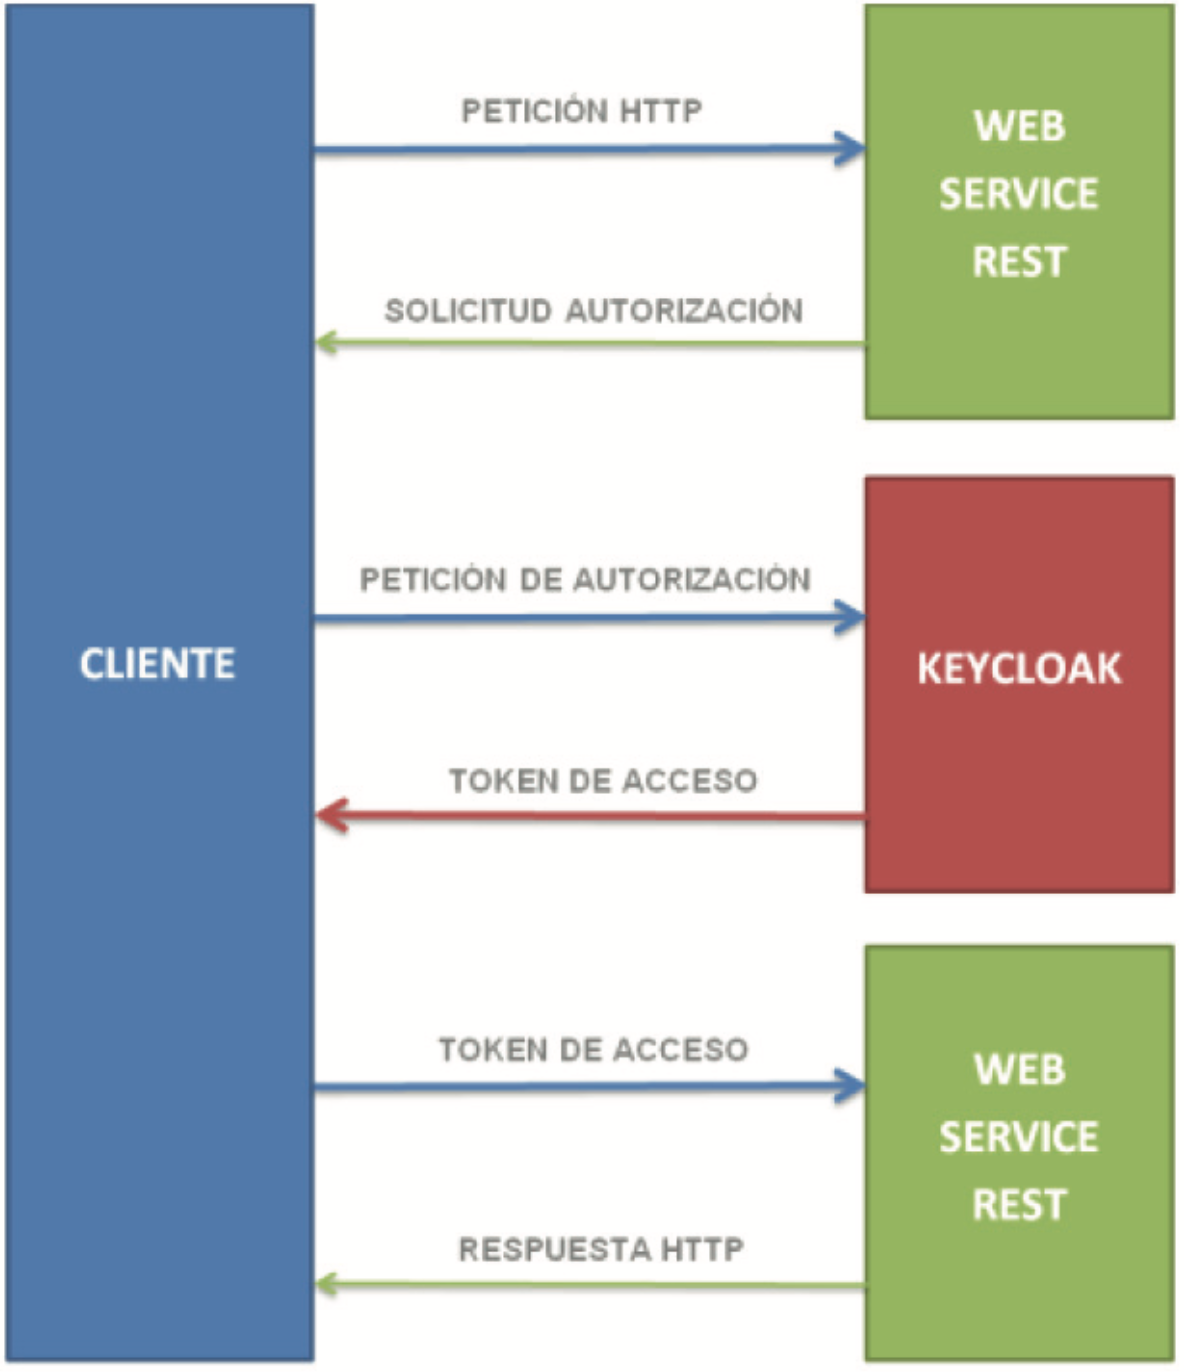
\includegraphics[width=0.7\linewidth]{Graphics/keycloak_info_flux}
	\caption{Flujo de Información en Keycloak}
	\label{fig:Flujo de Información en Keycloak}
\end{figure}

Este flujo asegurar que solo los usuarios a los que se les otorgó el acceso al servicio web puedan consumir dicha API. De esta forma se evita el acceso no autorizado a información que se transmite bajo un protocolo no seguro como lo es el protocolo HTTP. [\cite{muyon2020metodos}]
